%!TEX root=masterproef.tex

\chapter{Simulatie van routering voor een XBee-gebaseerd maasnetwerk}
\label{virtual-mesh}

Het hardwareplatform, beschreven in \ref{hardware-platform}, beschikt over een
XBee module om het ZigBee netwerk op te bouwen. Deze module biedt een zeer
hoogniveau interface aan, waardoor alle routering en andere lagerniveau
concepten verborgen blijven. Zo is het bv. onmogelijk om communicatie die niet
voor de eigen radio bestemd is op te vangen, terwijl dit net een typische
eigenschap is van een draadloos (maas)netwerk.

Aangezien het kunnen opvolgen van het verder doorsturen van berichten een
belangrijk aspect is en hiervoor alle communicatie die opgevangen kan worden
ter beschikking moet staan van het algoritme, was het nodig om dit gedrag na te
bootsen om een realistische demonstratie van de algoritmen mogelijk te maken.

Hiertoe werd een virtuele routering ge\"implementeerd. Deze maakt het mogelijk
om aan de hand van \emph{broadcast} berichten en extra informatie omtrent de
oorspronkelijke zender en eventuele tussenliggende knopen, alle mogelijkheden
van een volledig toegankelijk ZigBee netwerk te simuleren.

\section{Opstelling}

Figuur \ref{fig:xbee-setup} toont de opstelling voor de demonstratie: drie XBee
modules zijn geconfigureerd als een eind-knoop, een router en een
co\"ordinator. De co\"ordinator is via een \emph{explorerboard} verbonden met
een computer. Op deze manier is het mogelijk om deze XBee module te benaderen
aan de hand van een seri\"ele verbinding. De eind-knoop en de router zijn twee
identieke sensorknopen.

\begin{figure}[ht]
  \centering
  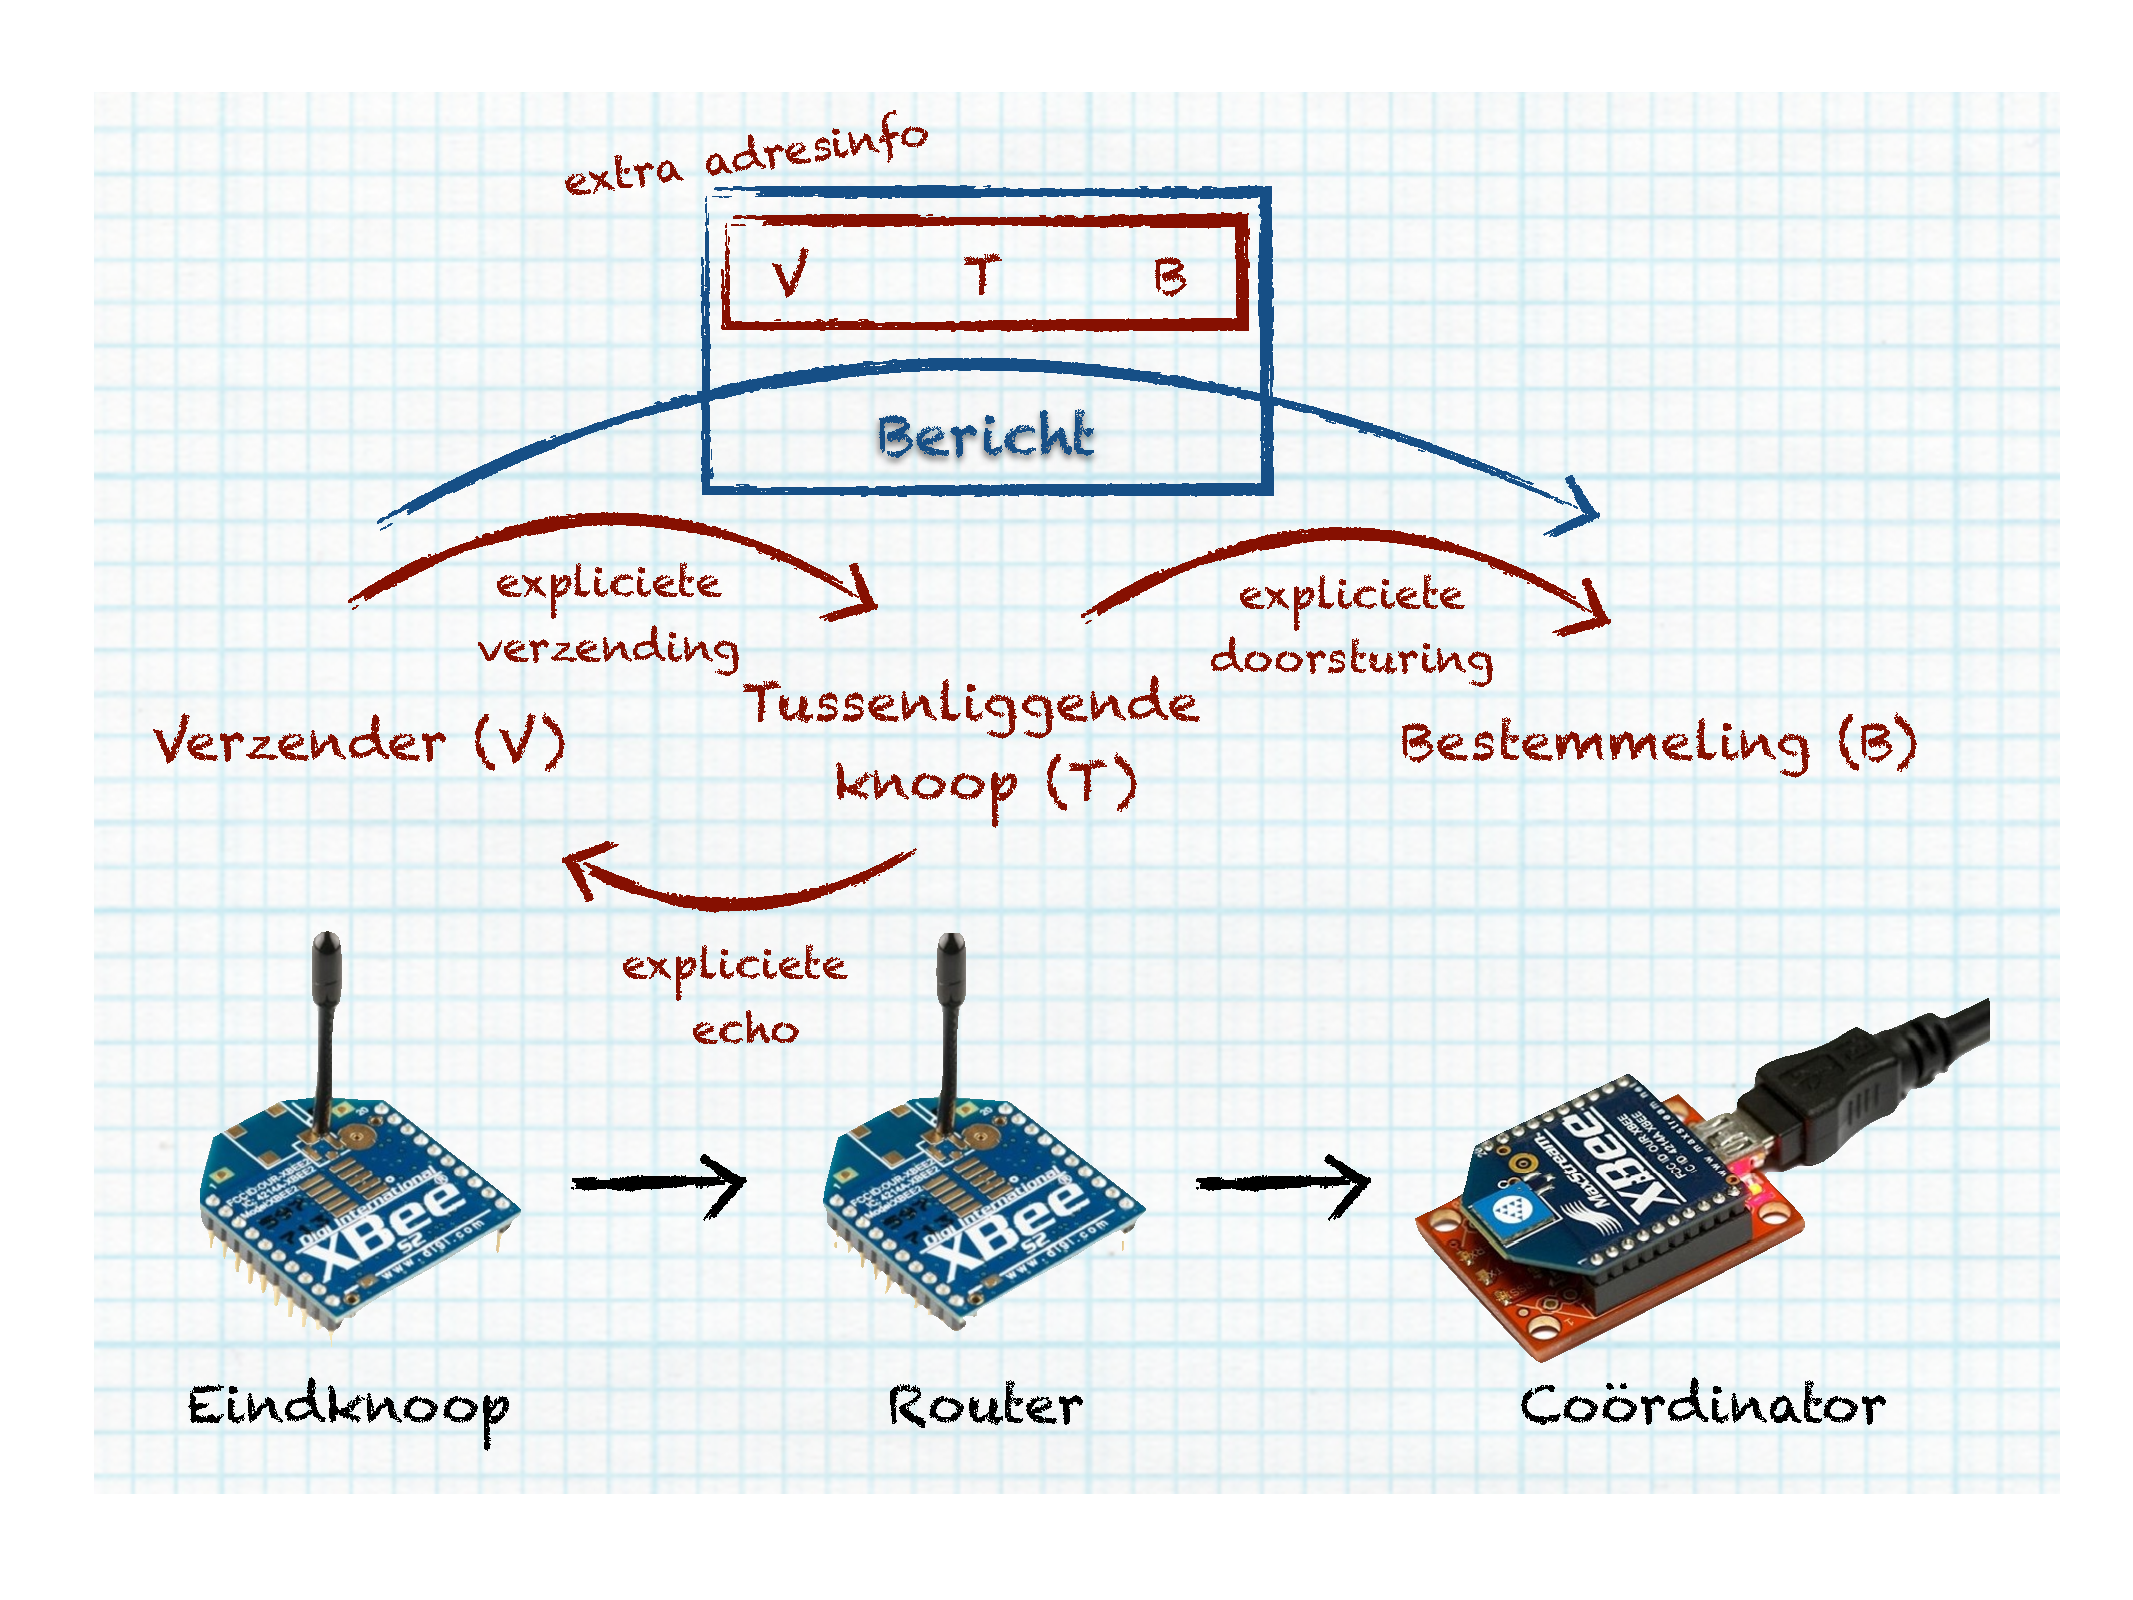
\includegraphics[width=\linewidth]{resources/xbee-setup.pdf}
  \caption{Opstelling van maasnetwerk voor demonstratie.}
  \label{fig:xbee-setup}
\end{figure}

Om met de drie XBee modules op een correcte manier tot een maasnetwerk te
komen, moeten we de modules voorzien van een specifieke configuratie. Zo wordt
bij de co\"rdinator de tijdspanne dat nieuwe knopen het netwerk kunnen
vervoegen beperkt tot \'e\'en minuut. Dit gebeurt aan de hand van het \ttt{NJ}
(Node Join) commando. Gedurende deze periode kan dan de router geactiveerd
worden. Na associatie van deze radio en het verstrijken van de minuut, kan dan
de eind-knoop geactiveerd worden. Deze zal niet meer rechtstreeks bij de
co\"ordinator kunnen aansluiten en zal via de router het netwerk moeten
benaderen.

\section{Doorsturen van berichten}

Een tweede aanpassing die dient doorgevoerd te worden, is de manier waarop de
router berichten van de eind-knoop verder doorstuurt naar de co\"ordinator.
Indien we dit door de standaard netwerkvoorzieningen van de XBee module zouden
later doen, zouden we deze berichten opnieuw niet kunnen onderscheppen. We
moeten deze daarom zelf \emph{manueel} doorsturen.

Bij het versturen van berichten worden tevens drie bijkomende netwerk adressen
van de betrokken knopen toegevoegd aan het feitelijke bericht: het adres van de
oorspronkelijke verzender, het adres van de tussenliggende knoop en het adres
van de uiteindelijke bestemmeling. Dit stelt ons functioneel in staat om
voldoende informatie te hebben om berichten van andere knopen onderling te
interpreteren.

De extra code die deze simulatie realiseert is weergegeven in listing
\ref{lst:virtual-mesh}. Ze volgt de opbouw van de overeenkomstige code voor
normale aansturing van de XBee module: een verzend functie, een ontvang functie
en de mogelijkheid om een externe verwerker voor binnenkomende berichten te
registreren.

De werking wordt duidelijk aan de hand van een voorbeeld, waarbij zowel de
eind-knoop als de router een bericht verzenden naar de co\"ordinator. De
uitvoer van deze demonstratie is weergegeven in figuur \ref{fig:virtual-mesh}:
van boven naar onder zien we de uitvier van de eind-knoop, de router en de
co\"ordinator.

Zowel de eind-knoop als de router gebruiken exact dezelfde code. Na het
initialiseren van de seri\"ele verbinding en het opzetten van de
netwerkassociatie, tonen beide knopen eerst hun eigen netwerk adres en dat van
hun hi\"erarchisch ouderlijke knoop (Engels: \emph{parent}). In dit geval heeft
de eind-knoop netwerk adres \ttt{4d 83} en de router adres \ttt{fa 7d}. We zien
dat de eind-knoop inderdaad als \emph{parent} de router opgeeft.

De router geeft als \emph{parent} \ttt{ff fe} aan. Dit adres staat voor een
onbekend adres. XBee routers geven dit adres standaard terug aangezien het
\emph{parent} concept voor hen niet bestaat. 

\inputminted[linenos,frame=lines,framesep=2mm,fontsize=\footnotesize,firstline=39, firstnumber=39]{c}{../src/demo/lib/network.c}
\vspace{-5mm}
\captionof{listing}{Simulatie van een maasnetwerk met XBee modules.
\label{lst:virtual-mesh}}
\vspace{3mm}

In deze beperkte simulatieopstelling kunnen we dit adres gelijkstellen aan het
adres van de co\"ordinator: \ttt{00 00}.

De router zal na associatie met het netwerk, gedurende 20 seconden wachten,
alvorens zijn eigen bericht te versturen. Gedurende deze tijd kunnen we de
eind-knoop activeren. Tijdens het wachten, verwerkt de router wel binnenkomende
berichten. Zoals we kunnen zien was de eind-knoop reeds verbonden met het
netwerk via de router na een 18tal seconden. De router ontving het bericht van
de eind-knoop en besliste op basis van de uiteindelijke bestemming om het
bericht verder te versturen. Dit expliciet doorgestuurde bericht komt zowel toe
bij de co\"ordinator als de eind-knoop.

Tot slot, verstuurt ook de router een bericht naar de co\"ordinator. Opnieuw
ontvangen zowel de co\"ordinator als de eind-knoop dit bericht.

\begin{figure}[ht]
\centering
\begin{subfigure}{.67\linewidth}
  \centering
  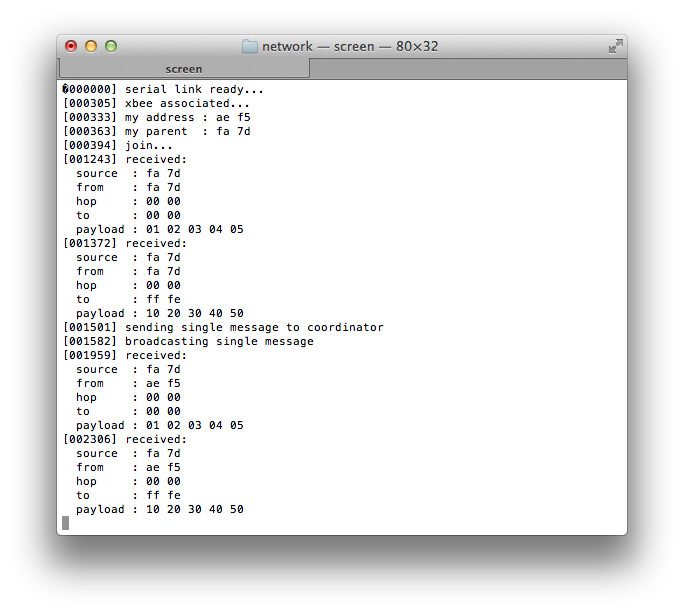
\includegraphics[width=.9\linewidth]{../src/demo/network/end-device.png}
  \caption{Eind-knoop}
  \label{fig:virtual-mesh-end-device}
\end{subfigure}
\begin{subfigure}{.67\linewidth}
  \centering
  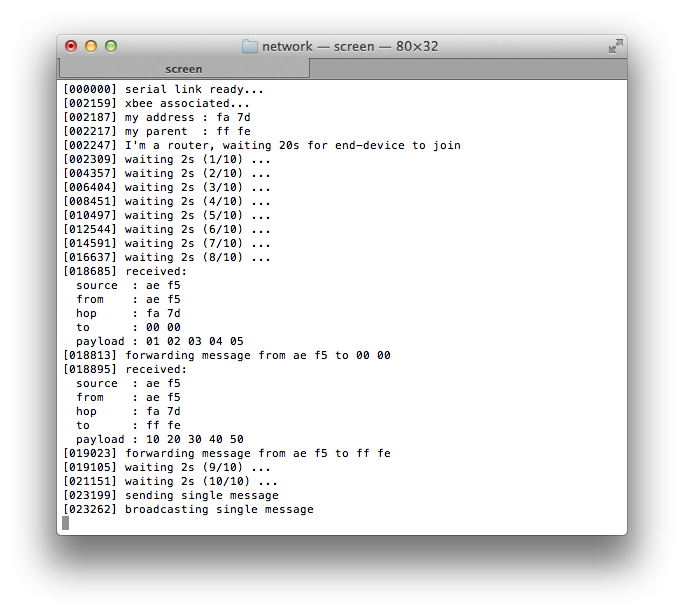
\includegraphics[width=.9\linewidth]{../src/demo/network/router.png}
  \caption{Router}
  \label{fig:virtual-mesh-router}
\end{subfigure}
\begin{subfigure}{.67\linewidth}
  \centering
  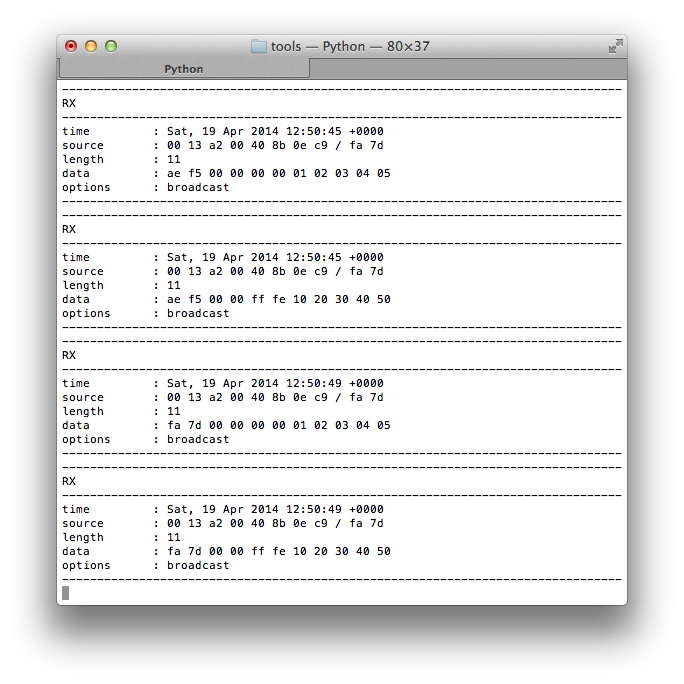
\includegraphics[width=.9\linewidth]{../src/demo/network/coordinator.png}
  \caption{Coordinator}
  \label{fig:virtual-mesh-coordinator}
\end{subfigure}
\caption{Simulatie van een maasnetwerk op basis van XBee modules.}
\label{fig:virtual-mesh-output}
\end{figure}
